\documentclass[tikz,dvisvgm,border=0pt]{standalone}
% Shared look for every Tokimeki figure.
\usepackage[T1]{fontenc}
\usepackage{lmodern}
\usetikzlibrary{arrows.meta,calc,backgrounds,patterns}
\renewcommand{\familydefault}{\sfdefault}

\definecolor{ink}{HTML}{1F2D33}
\definecolor{muted}{HTML}{7A8A8C}
\definecolor{rule}{HTML}{A7B6B8}
\definecolor{diskfill}{HTML}{EEF1F0}
\definecolor{diskline}{HTML}{8FA3A5}
\definecolor{runfill}{HTML}{E3F2EC}
\definecolor{runline}{HTML}{3E8C70}
\definecolor{userfill}{HTML}{FFF1E0}
\definecolor{userline}{HTML}{C9843E}
\definecolor{orangefill}{HTML}{FCDDBA}
\definecolor{orangeline}{HTML}{D27F2F}
\definecolor{bluefill}{HTML}{D6E4F5}
\definecolor{blueline}{HTML}{4F7FB3}
\definecolor{redline}{HTML}{C0453A}
\definecolor{purplefill}{HTML}{E7DDF3}
\definecolor{purpleline}{HTML}{8462B3}

\tikzset{
  every node/.style={text=ink, font=\small},
  fig/.style={show background rectangle, background rectangle/.style={fill=white}, inner frame sep=12pt},
  % places
  disk/.style={draw=diskline, line width=0.9pt, fill=diskfill},
  runner/.style={draw=runline, line width=1pt, fill=runfill},
  user/.style={draw=userline, line width=1pt, fill=userfill},
  title/.style={font=\bfseries\small, anchor=north west},
  where/.style={font=\footnotesize, text=muted, anchor=north west},
  % things
  card/.style={draw=rule, line width=0.8pt, fill=white,
               minimum width=1.9cm, minimum height=0.62cm, inner sep=2pt, font=\ttfamily\scriptsize},
  groupA/.style={card, draw=orangeline, fill=orangefill},
  groupB/.style={card, draw=blueline, fill=bluefill},
  groupC/.style={card, draw=purpleline, fill=purplefill},
  slot/.style={draw=runline!55, line width=0.8pt, dash pattern=on 2.5pt off 1.8pt, fill=white,
               minimum width=2.1cm, minimum height=0.8cm},
  cmd/.style={fill=ink, text=white, font=\ttfamily\scriptsize, inner sep=4pt, anchor=south west},
  % arrows: solid = write a file, dashed = read a file
  write/.style={-{Stealth[length=6.5pt,width=5.5pt]}, line width=1.2pt},
  read/.style={-{Stealth[length=6.5pt,width=5.5pt]}, line width=1.1pt, dash pattern=on 4pt off 2.5pt},
  lbl/.style={font=\footnotesize, fill=white, inner sep=1.5pt},
  num/.style={circle, fill=ink, text=white, font=\bfseries\scriptsize, inner sep=1pt, minimum size=12pt},
}

% \diskslab{x0}{y0}{x1}{y1}  -- the shared directory every node mounts
\newcommand{\diskslab}[4]{%
  \draw[disk] (#1,#2) rectangle (#3,#4);
  \node[font=\bfseries\footnotesize, text=diskline, anchor=south east] at (#3-0.15,#2+0.08)
    {shared filesystem};
}

% \machine{x0}{y0}{x1}{y1}{label} -- a physical node: white box with a dark header bar
\newcommand{\machine}[5]{%
  \draw[ink, line width=1pt, fill=white] (#1,#2) rectangle (#3,#4);
  \fill[ink] (#1,#4-0.5) rectangle (#3,#4);
  \fill[ink] (#1,#4-0.5) rectangle (#3,#4-0.3);
  \node[font=\bfseries\footnotesize, text=white, anchor=west] at (#1+0.15,#4-0.25) {#5};
}
% \proc{x0}{y0}{x1}{y1}{label} -- the runner daemon running on a node
\newcommand{\proc}[5]{%
  \draw[runner] (#1,#2) rectangle (#3,#4);
  \node[font=\bfseries\scriptsize, text=runline, anchor=north west] at (#1+0.1,#4-0.05) {#5};
}
% \tray{x0}{y0}{x1}{y1}{label} -- a place on the shared filesystem
\newcommand{\tray}[5]{%
  \draw[draw=rule, fill=white] (#1,#2) rectangle (#3,#4);
  \node[font=\footnotesize, text=muted, anchor=north east] at (#3-0.08,#4-0.03) {#5};
}
\tikzset{
  script/.style={draw=ink, line width=0.8pt, fill=white, font=\ttfamily\scriptsize,
                 minimum width=1.7cm, minimum height=1.0cm, inner sep=2pt,
                 append after command={\pgfextra{\let\n\tikzlastnode}
                   (\n.north east) ++(-0.28,0) -- ++(0,-0.28) -- ++(0.28,0)}},
}

\begin{document}
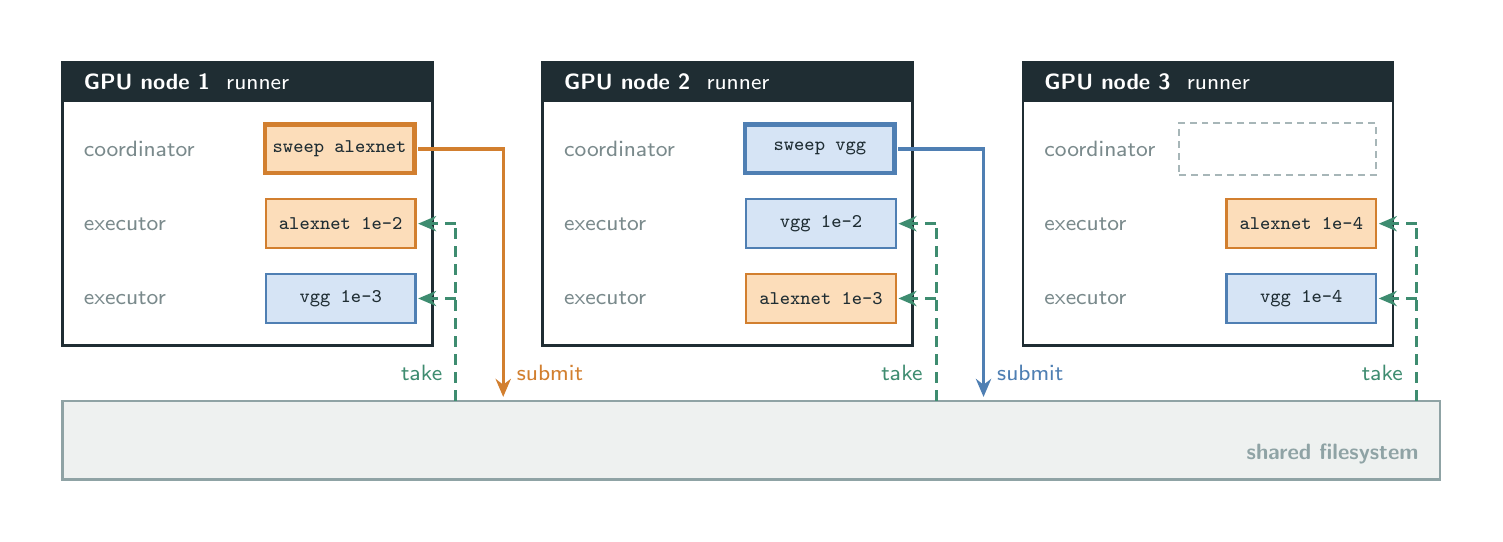
\begin{tikzpicture}[fig]
  \tikzset{job/.style={card, minimum width=2.5cm, minimum height=0.66cm, anchor=east},
           free/.style={job, draw=rule, dash pattern=on 2.5pt off 1.8pt, fill=white},
           role/.style={font=\footnotesize, text=muted, anchor=west}}

  \diskslab{0}{0.9}{17.5}{1.9}

  % \gpunode{n}{x}{coordinator style}{coordinator text}{exec 1 style}{exec 1}{exec 2 style}{exec 2}
  \newcommand{\gpunode}[8]{%
    \machine{#2}{2.6}{#2+4.7}{6.2}{GPU node #1 \ \normalfont runner}
    \node[role] at (#2+0.15,5.1) {coordinator};
    \node[role] at (#2+0.15,4.15) {executor};
    \node[role] at (#2+0.15,3.2) {executor};
    \node[#3] at (#2+4.5,5.1) {#4};
    \node[#5] at (#2+4.5,4.15) {#6};
    \node[#7] at (#2+4.5,3.2) {#8};
    % executors take trials from the shared filesystem
    \draw[read, draw=runline, -] (#2+5.0,1.9) -- (#2+5.0,4.15);
    \draw[read, draw=runline] (#2+5.0,4.15) -- (#2+4.52,4.15);
    \draw[read, draw=runline] (#2+5.0,3.2) -- (#2+4.52,3.2);
    \node[font=\footnotesize, text=runline, anchor=east] at (#2+4.95,2.25) {take};
  }
  \gpunode{1}{0}{job, groupA, line width=1.6pt}{sweep alexnet}{job, groupA}{alexnet 1e-2}{job, groupB}{vgg 1e-3}
  \gpunode{2}{6.1}{job, groupB, line width=1.6pt}{sweep vgg}{job, groupB}{vgg 1e-2}{job, groupA}{alexnet 1e-3}
  \gpunode{3}{12.2}{free}{}{job, groupA}{alexnet 1e-4}{job, groupB}{vgg 1e-4}

  % the two coordinators submit their trials
  \foreach \x/\c in {0/orangeline, 6.1/blueline} {
    \draw[write, draw=\c] (\x+4.52,5.1) -- (\x+5.6,5.1) -- (\x+5.6,1.95);
    \node[font=\footnotesize, text=\c, anchor=west] at (\x+5.65,2.25) {submit};
  }
\end{tikzpicture}
\end{document}
